\chapter{大质量恒星的命运}
\section{大质量恒星的主序后演化}
前面提到大质量恒星的演化相较中等质量和小质量恒星要顺利的多,每一步点燃温度都能直接达到,随后进行一步步的核反应,最终能生成铁核。

同时也因为温度高,大质量恒星的核反应速率非常快,演化速率也非常快,并且伴随着剧烈的星风,和较大的质量损失率。

\begin{figure}[hbt]
  \centering
  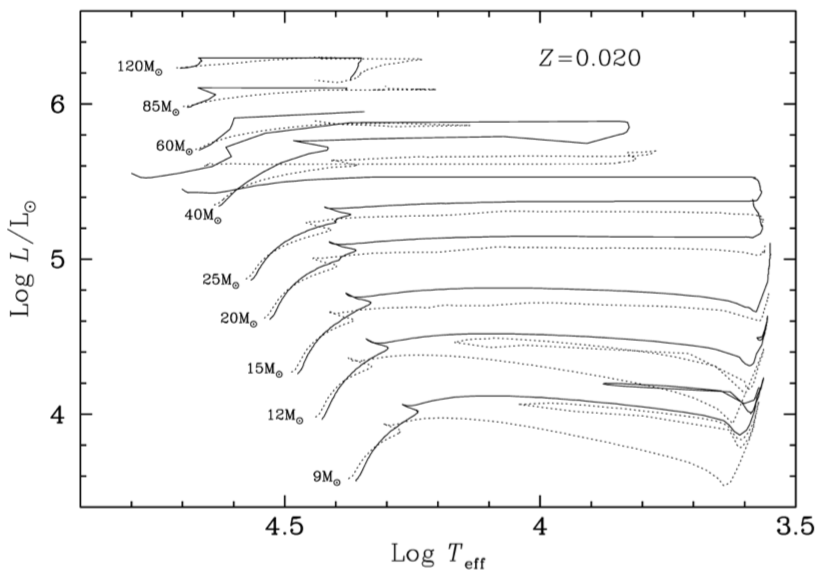
\includegraphics[width=10cm]{chapters/15/massive}
  \caption{大质量恒星的演化轨迹。实线考虑自转,虚线不考虑自转。}
  \label{}
\end{figure}

\section{超新星}
铁核形成后,因为铁的核反应过程是一个吸热过程,因此恒星无法继续平衡,最终导致恒星塌缩,然后发生超新星爆发。超新星爆发会抛离恒星的外层物质,留下中心的简并核,根据核的质量不同,分别会形成白矮星、中子星和黑洞。

在超新星爆发过程中,比铁更重的元素会被生成。宇宙中的超新星爆发来源并不是只有大质量恒星的塌缩,不同的来源会导致它的光谱也不同,因此人们根据以下几个原则对超新星进行分类,详细分类见图\ref{fig:supernova}:
\begin{itemize}
  \item 有无氢线,无氢线的超新星由于最早被发现,被定义为I型超新星,有氢线为II型超新星
  \item 有无硅线,I型超新星中有硅线的为Ia型,无硅线为Ib和Ic
\end{itemize}

\begin{figure}[hbt]
  \centering
  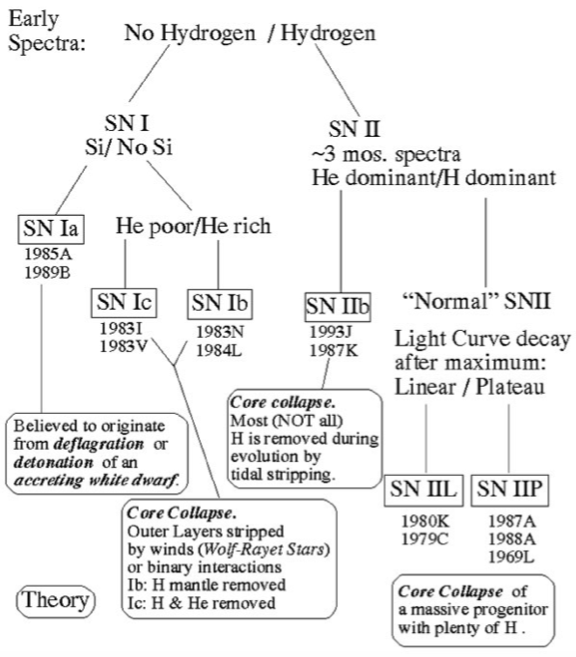
\includegraphics[width=10cm]{chapters/15/supernova}
  \caption{超新星的详细分类}
  \label{fig:supernova}
\end{figure}

\section{伽马射线暴}
上世纪美苏冷战期间,为了监视苏联的核试验,美国发射了卫星来探测苏联的伽马射线源,却因此意外地发现了\textbf{伽马射线暴}现象。通过对伽马射线暴的长时间检测,人们发现它们在天空中的分布几乎是均匀的,因此确定它们的来源主要是\textbf{银河系以外}。

伽马射线暴主要表现为天空中某个方向的伽马射线强度突然出现短暂峰值,当天文学家把观测到的伽马射线线按照持续时间分类后发现,它们以2\,s为界明显分为两类——\textbf{长暴和短暴},其中短暴能量高,长暴能量低。